\section{Naxsi}

%%%%%%% SECTION 1/3
\begin{frame}
  \frametitle{What is a Naxsi?}
   \begin{itemize}
   \item Nginx Anti Xss \& Sql Injection
   \item Web Application Firewall
   \item Module Nginx webserver
   \item Designed as reverse proxy
  \end{itemize}
\end{frame}

\begin{frame}
  \frametitle{Naxsi request flow}
    \begin{center} 
      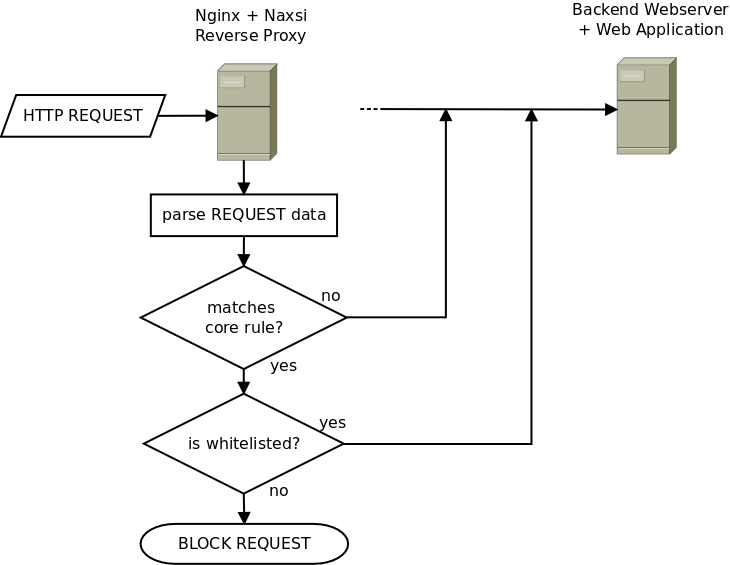
\includegraphics[width=0.75\textwidth]{../paper/images/request_flow.png}
    \end{center}
\end{frame}


\begin{frame}
  \frametitle{Whitelist processing}
    \begin{itemize}
     \item HTTP requests parsed
      \begin{itemize}
        \item devided into zones:
	\item ARGS (GET arguments), URL (the full URI), BODY (POST arguments), as well as Cookie http header
      \end{itemize}
      \item Core rules
      \begin{itemize}
        \item RegEx
	\item unique IDs
      \end{itemize}
     \item White lists and Specific Rules
       \begin{itemize}
        \item define strictness
      \end{itemize}
  \end{itemize}
\end{frame}

\section{Research questions}

\begin{frame}
  \frametitle{Research Question(s)}
   \begin{center}
   \LARGE{"How does Naxsi influence the performance of the Nginx webserver?"}
  \end{center}
\end{frame}

\begin{frame}
  \frametitle{Research Question(s)}
   \begin{center}
   \LARGE{"What is the performance of Nginx firewall when Naxsi is isolated?"}
   \vskip1em
   \LARGE{"What is the performance of the Nginx firewall in a real life scenario?"}
  \end{center}
\end{frame}

\begin{frame}
  \frametitle{Experimental setup}
    \begin{center} 
      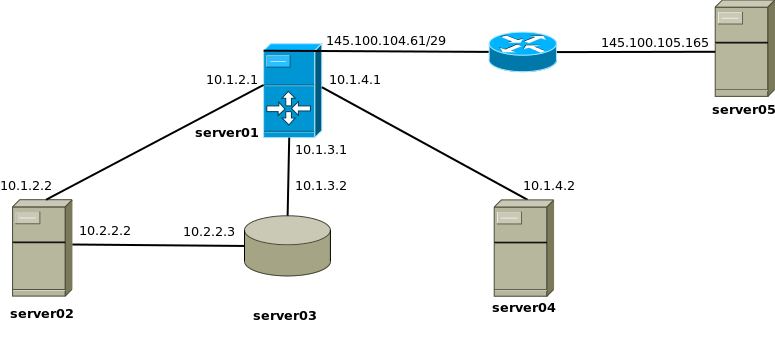
\includegraphics[width=0.80\textwidth]{../paper/images/infrastructure.png}
    \end{center}
\end{frame}
